\chapter{Seznámení s aplikací a databází}
\label{3-seznameni-s-aplikaci-a-databazi}

\section{Navázání na projekt FGIS}

Tato diplomová práce navazuje na započatý projekt z předmětu Free
Software GIS. Na projektu se také podílel autor práce. 
Projekt měl za úkol vytvořit jednoduchou webovou aplikaci, kdy
přihlášení uživatelé mohli zobrazovat, vytvářet, editovat a mazat záznamy
z databáze. Databáze pro tento projekt byla pouze cvičná a obsahovala
pouze několik tabulek s textovými poli. Projekt ovšem nebyl zcela
dokončen, protože se nepovedlo vytvořit všechny funkce tak, aby
správně fungovali. Data do databáze šla přidávat, zobrazovat je a 
mazat, ale při editaci se po uložení nepřepsala aktuální data v
databázi.

\begin{figure}[H] \centering
    
\includegraphics[width=400pt]{./pictures/4-nahled-menu-fgis.PNG}
    \caption[Náhled aplikace vytvořené v projektu FGIS]{Náhled aplikace vytvořené v projektu FGIS}
	\label{fig:Náhled aplikace}              
\end{figure}
 
 \section{Zkušební databáze}
 
Na začátku projektu byla používána pouze zkušební databáze, jejíž použití 
bylo z důvodu neznalosti přesné struktury finální databáze. Zkušební databáze 
sloužila na začátku projektu pro inicializaci aplikace, a vytvoření základních 
funkcionalit. Databáze obsahovala pouze tabulku s textovými daty.

 \newpage

\section{Centrální databáze}
\label{centralni-db}
Databáze fondů Národního muzea obsahuje objekty, které se budou ve 
vyvíjené aplikaci zobrazovat a budou rozšířena o další data. Všechna data 
v této databázi jsou obsažena v jedná tabulace. Část sloupců v této tabulce 
obsahuje informace o objektu a část o obrázku, který je k němu přidělen. 
Jednotlivé objekty ovšem disponují více obrázky, kdy se pro každý obrázek
vytváří nový databázový záznam. Zde dochází k duplikování velké části dat, 
kdy se sloupce s informacemi o objektu kopírují a mění se pouze část s 
obrázky a jejich metadaty. Databáze je tedy v nenormalizované formě.

\begin{figure}[H] \centering
    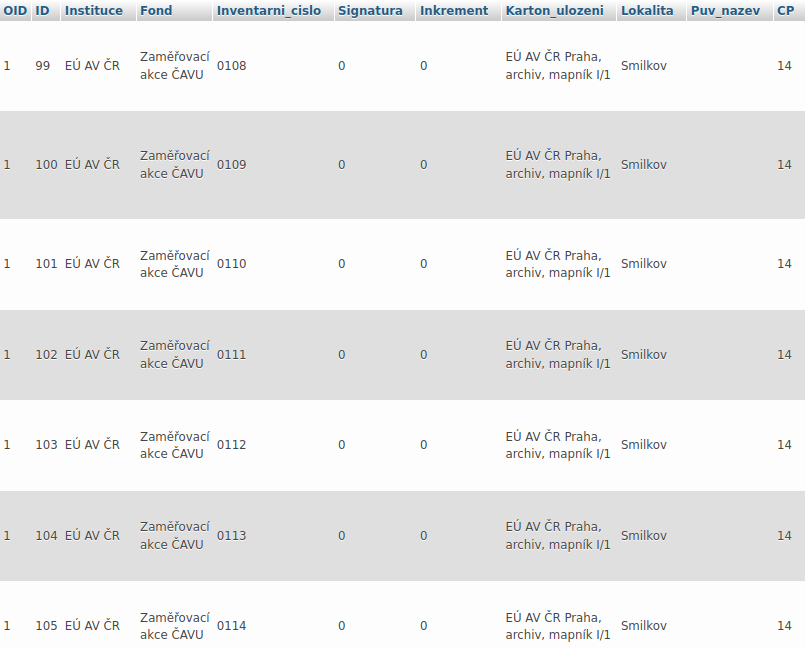
\includegraphics[width=420pt]{./pictures/5-ukazka-basedata.PNG}
    \caption[Náhled dat z centrální databáze s viditelnými duplicitami]{Náhled dat centrální z databáze s viditelnými duplicitami}
	\label{fig:Náhled dat z centrální databáze s viditelnými duplicitami}              
\end{figure}


